\documentclass[10pt,aspectratio=169]{beamer}

% --- packages -------------------------------------------------------------
\usepackage{amsmath,amssymb,amsthm}
\usepackage{mathtools}
\usepackage{bm}
\usepackage{upgreek}
\usepackage{graphicx}
\usepackage{epstopdf}   % so the .eps figures compile under pdflatex
\usepackage{xcolor}
\usepackage{booktabs}

% --- theme ---------------------------------------------------------------
\usetheme{Madrid}
\usecolortheme{seahorse}
\useinnertheme{circles}
\useoutertheme{infolines}
\setbeamertemplate{navigation symbols}{}
\setbeamerfont{frametitle}{size=\large}

% --- shortcuts -----------------------------------------------------------
\newcommand{\gd}{{\dot{\bm{\gamma}}}}
\renewcommand{\Re}{\operatorname{Re}}
\newcommand{\De}{\operatorname{De}}
\newcommand{\Renx}{\Re_{n,x}}

% --- title block --------------------------------------------------------
\title[Carreau Boundary Layers]{On Self-Similar Viscosity Models for\\ Carreau Boundary Layer Flows}
\author[Reinberger, Barlow, Weinstein]{W.~Cade Reinberger \and Nathaniel S.~Barlow \and Steven J.~Weinstein}
\institute[RIT]{School of Mathematics and Statistics\\ \&\ Department of Chemical Engineering\\ Rochester Institute of Technology}
\date{\today}

\begin{document}

% =========================================================================
\begin{frame}
  \titlepage
\end{frame}

% =========================================================================
\begin{frame}{Outline}
  \begin{enumerate}
    \item Motivation: boundary layers in coating-flow applications
    \item Rheological models: Newtonian, power-law, Carreau
    \item Formulation and (pseudo-)similarity
    \item \textbf{New} power-law Sakiadis solutions for $\alpha<\tfrac{1}{2}$ and $\alpha>1$
    \item Wall shear: comparing self-similar predictions to Carreau
    \item A simple criterion for combining similarity solutions
    \item Conclusions
  \end{enumerate}
\end{frame}

% =========================================================================
\begin{frame}{Motivation}
  \begin{columns}[T,onlytextwidth]
    \column{0.55\textwidth}
      \textbf{Boundary layers} are thin, viscosity-dominated regions adjacent to a wall.
      \vspace{0.5em}

      Two canonical flat-wall problems:
      \begin{itemize}
        \item \textbf{Blasius (1908)} --- fluid moves over a stationary wall.
        \item \textbf{Sakiadis (1961)} --- wall moves through stationary fluid.
      \end{itemize}
      \vspace{0.5em}

      Sakiadis flows are directly relevant to \emph{liquid film coating}, fiber drawing, and other industrial processes.
      \vspace{0.5em}

      Real coating fluids are \emph{non-Newtonian} --- their viscosity depends on shear rate.

    \column{0.45\textwidth}
      \begin{center}
        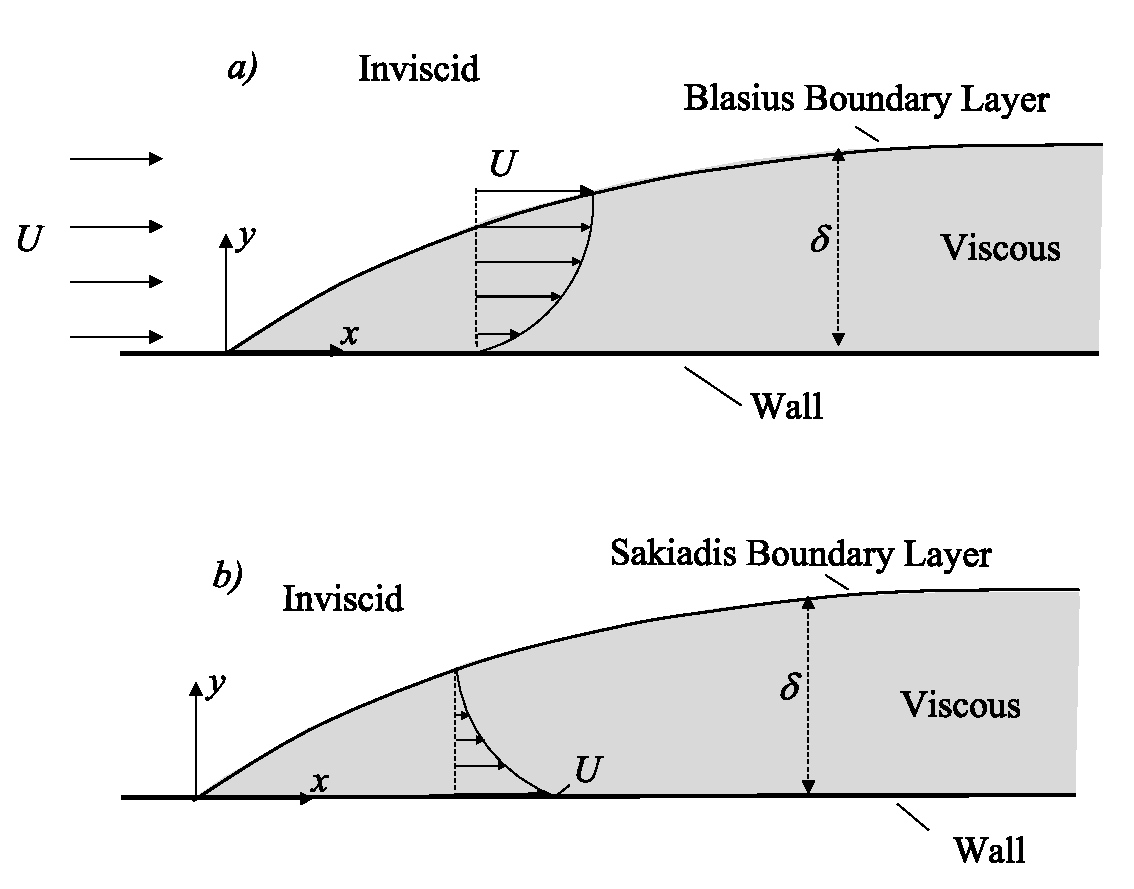
\includegraphics[width=\linewidth]{schematics_pdf_cropped.pdf}
      \end{center}
  \end{columns}
\end{frame}

% =========================================================================
\begin{frame}{Why Care About the Full Rheological Profile?}
  \begin{columns}[T,onlytextwidth]
    \column{0.45\textwidth}
      A single boundary layer flow accesses a \emph{wide range} of strain-rate magnitudes:
      \begin{itemize}
        \item Near the wall: $|\gd|$ is large.
        \item Far from the wall: $|\gd|\to 0$.
        \item Far downstream: $|\gd|$ decreases as the boundary layer grows.
      \end{itemize}
      \vspace{0.5em}
      So the \emph{whole rheological curve} can matter --- not just the power-law region.

    \column{0.55\textwidth}
      \begin{center}
        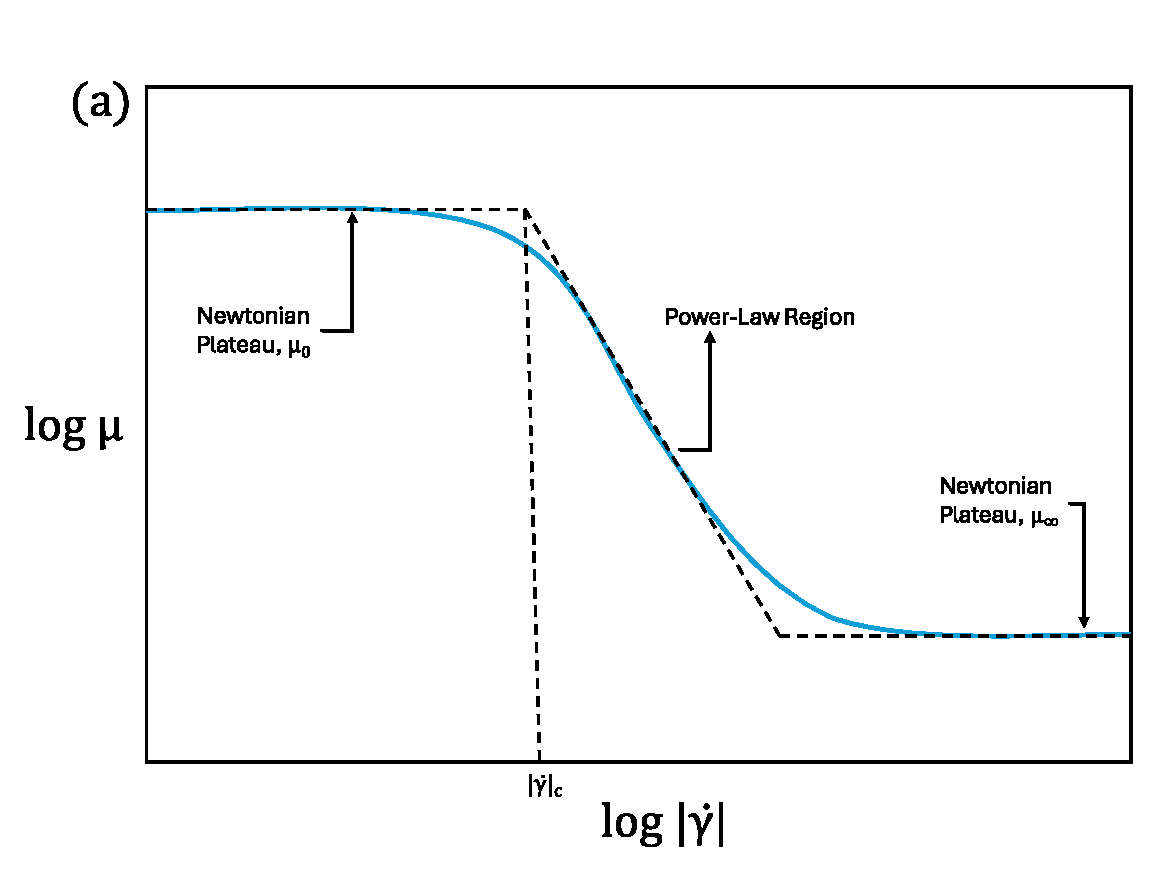
\includegraphics[width=0.49\linewidth]{rheo_thin_cropped_rotated.pdf}\hfill
        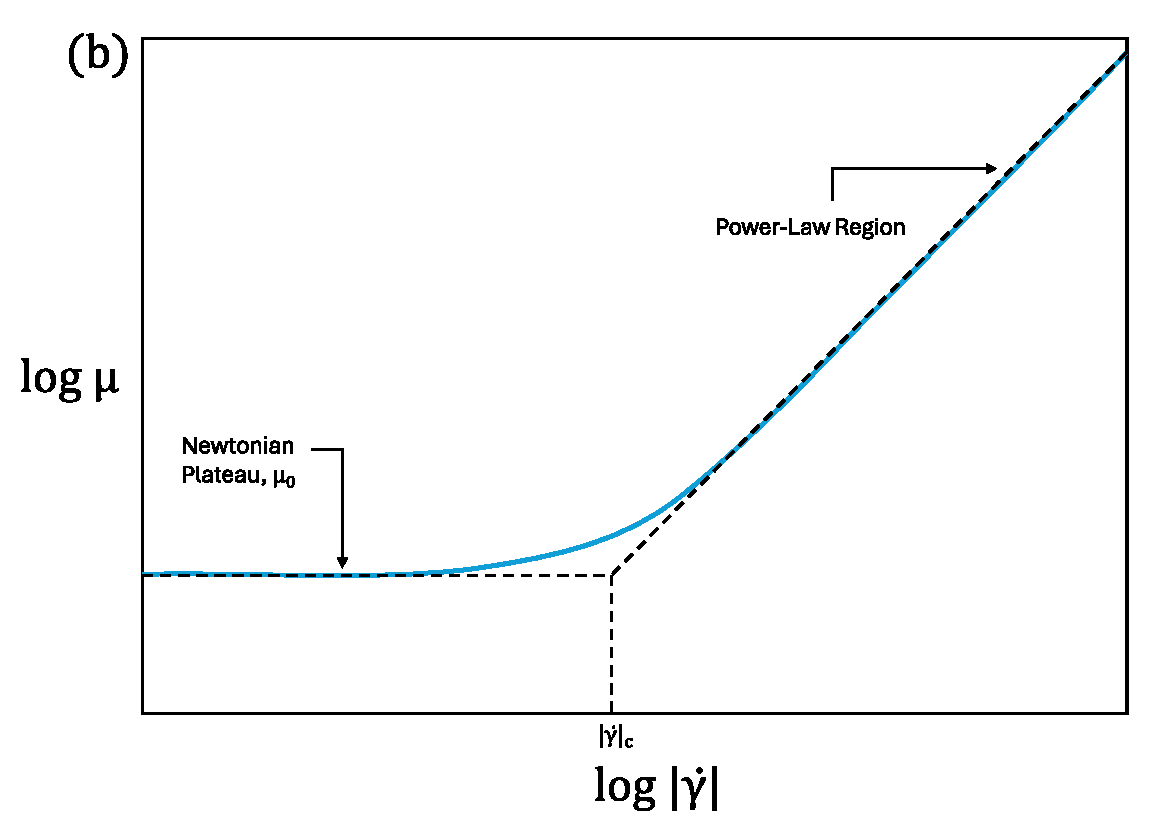
\includegraphics[width=0.49\linewidth]{rheo_thick_cropped_rotated.pdf}
      \end{center}
      \footnotesize
      \textbf{Left:} shear-thinning. \textbf{Right:} shear-thickening.\\
      Solid: Carreau. Dashed: power-law and Newtonian asymptotes.
  \end{columns}
\end{frame}

% =========================================================================
\begin{frame}{Three Viscosity Models}
  \textbf{Power-law (Ostwald--de Waele).}
  \[
    \mu = K\,|\gd|^{\alpha-1}.
  \]
  Captures shear-thinning ($\alpha<1$) or shear-thickening ($\alpha>1$); admits similarity solutions.\\
  \emph{But:} $\mu\to\infty$ or $\mu\to0$ in unphysical limits.
  \vspace{0.7em}

  \textbf{Carreau (with $\mu_\infty=0$).}
  \[
    \mu = \mu_0\!\left(1+(\lambda|\gd|)^2\right)^{(\alpha-1)/2}.
  \]
  Smoothly connects a Newtonian plateau at low $|\gd|$ to power-law behavior at high $|\gd|$.\\
  \emph{Cost:} no exact similarity solution.
  \vspace{0.7em}

  \textbf{Connecting them:}\quad $K=\mu_0\lambda^{\alpha-1}$,\quad $|\gd|_c = 1/\lambda$.
\end{frame}

% =========================================================================
\begin{frame}{Question for This Talk}
  \begin{block}{Central question}
    How well do the simpler, \emph{self-similar} Newtonian and power-law solutions
    describe the boundary layer of a Carreau fluid, and \emph{when} can they be used in place of it?
  \end{block}
  \vspace{0.5em}
  \textbf{Metric:} wall shear rate $\bar\tau = \tau/(\rho U^2)$.
  \vspace{0.5em}

  \textbf{Two contributions:}
  \begin{enumerate}
    \item New self-similar Sakiadis power-law solutions for $\alpha<1/2$ and $\alpha>1$ ---
          previously believed not to exist.
    \item A quantitative comparison of wall-shear predictions across models, leading to a
          dimensionless criterion for combining similarity solutions to approximate the Carreau result.
  \end{enumerate}
\end{frame}

% =========================================================================
\begin{frame}{Boundary-Layer Formulation}
  Streamwise velocity $u_x$, transverse $u_y$, with $\tau_{yx}=\mu(|\gd|)\,\partial u_x/\partial y$:
  \[
    \frac{\partial u_x}{\partial x} + \frac{\partial u_y}{\partial y}=0,\qquad
    \rho\!\left(u_x\frac{\partial u_x}{\partial x} + u_y\frac{\partial u_x}{\partial y}\right) = \frac{\partial \tau_{yx}}{\partial y}.
  \]
  \vspace{0.3em}

  \begin{center}
  \begin{tabular}{lll}
    \toprule
    Location & Blasius & Sakiadis \\
    \midrule
    $y=0$         & $u_x=0,\; u_y=0$ & $u_x=U,\; u_y=0$ \\
    $y\to\infty$  & $u_x\to U$       & $u_x\to 0$       \\
    \bottomrule
  \end{tabular}
  \end{center}
  \vspace{0.5em}

  Pressure plays no role; boundary layer is driven entirely by relative wall--fluid motion.
\end{frame}

% =========================================================================
\begin{frame}{Power-Law Similarity Reduction}
  Substituting the standard similarity variables for a power-law fluid,
  \[
    \eta = y\!\left(\frac{\rho U^{2-\alpha}}{Kx}\right)^{\!1/(\alpha+1)}\!,\qquad
    f_p(\eta;\alpha) = \frac{\eta\,\psi}{Uy},
  \]
  reduces the PDE to a single ODE:
  \[
    \alpha(\alpha+1)\,f_p''' + f_p f_p''\,|f_p''|^{1-\alpha} = 0,
  \]
  with the BCs $f_p(0)=0$, $f_p'(0)=0$, $f_p'(\infty)\to1$ (Blasius) or
  $f_p'(0)=1$, $f_p'(\infty)\to0$ (Sakiadis).
  \vspace{0.4em}

  Wall shear rate (dimensional):
  \[
    \tau_p = K\!\left(U|f_p''(0;\alpha)|\!\left(\frac{\rho U^{2-\alpha}}{Kx}\right)^{\!1/(\alpha+1)}\right)^{\!\alpha}.
  \]
\end{frame}

% =========================================================================
\begin{frame}{Carreau ``Pseudo-Similarity''}
  No exact similarity exists, but following \emph{Griffiths et al.\ (2016)} we use the \emph{Newtonian}
  similarity variable; the $x$-dependence survives only as a parameter:
  \[
    \delta = \frac{\lambda^2 U^3 \rho}{\mu_0 x} = \frac{\De^2}{\Renx},
  \]
  giving a \emph{one-parameter family} of ODEs:
  \[
    \left(1+\alpha\delta f_c''^{\,2}\right)\!\left(1+\delta f_c''^{\,2}\right)^{\!(\alpha-3)/2} f_c''' + \tfrac{1}{2}f_c f_c'' = 0.
  \]
  \begin{itemize}
    \item One ODE solve per streamwise location $x$.
    \item $\delta$ acts as an effective relaxation time --- shrinks downstream as the boundary layer grows.
    \item Wall shear: $\;\tau_c = \sqrt{\rho\mu_0 U^3/x}\;f_c''(0;\delta)\bigl(1+\delta f_c''(0;\delta)^2\bigr)^{(\alpha-1)/2}.$
  \end{itemize}
\end{frame}

% =========================================================================
\begin{frame}{A Puzzling Gap in the Literature}
  For the Sakiadis power-law problem, prior work (Fox et al.\ 1969; Naghshineh et al.\ 2023)
  reports \emph{no solution} for
  \[
    \alpha < \tfrac{1}{2}\quad\text{or}\quad \alpha > 1.
  \]
  The argument assumed an asymptotic form $f_p \sim C + h(\eta)$ with $h\ll C$ as $\eta\to\infty$.
  The dominant balance gives
  \[
    f_p \sim C + D(1+E\eta)^{(2\alpha-1)/(\alpha-1)},\qquad \tfrac{1}{2}<\alpha<1,
  \]
  which fails self-consistency outside this window.
  \vspace{0.6em}

  \begin{block}{Resolution}
    The boundary condition $f_p'(\infty)\to 0$ does \emph{not} require $f_p\to C$.
    Allowing $f_p$ to grow algebraically opens up new admissible solutions.
  \end{block}
\end{frame}

% =========================================================================
\begin{frame}{New Asymptotic Form for $\alpha<1/2$}
  We propose
  \[
    f_p(\eta;\alpha)\sim H(\eta+J)^{p},\quad
    p=\frac{1-2\alpha}{2-\alpha},\quad
    H = \!\left(\frac{\alpha(\alpha+1)(2-p)}{p^{1-\alpha}(1-p)^{1-\alpha}}\right)^{\!1/(2-\alpha)}.
  \]
  \begin{columns}[T,onlytextwidth]
    \column{0.5\textwidth}
      Treating the BVP as an IVP in $\kappa=f_p''(0;\alpha)$:
      \begin{itemize}
        \item $\kappa>\kappa_p$: monotone, unbounded.
        \item $\kappa<\kappa_p$: nonmonotone, eventually decreases.
        \item \textbf{$\kappa=\kappa_p$:} a separatrix --- the unique trajectory smoothly approaching $f_p'\to 0$.
      \end{itemize}
    \column{0.5\textwidth}
      \begin{center}
        
\includegraphics[width=\linewidth]{fig3.eps}
      \end{center}
      \footnotesize Shooting solutions for $\alpha=0.3$.
  \end{columns}
\end{frame}

% =========================================================================
\begin{frame}{Verifying the Asymptotic}
  \begin{columns}[T,onlytextwidth]
    \column{0.55\textwidth}
      \begin{center}
        
\includegraphics[width=\linewidth]{new_thinning_asymptotic.eps}
      \end{center}
    \column{0.45\textwidth}
      Log--log plot of the separatrix solution ($\alpha=0.1$).
      \vspace{0.5em}

      \textbf{Solid:} numerical solution.\\
      \textbf{Dashed:} predicted $f_p\sim H(\eta+J)^p$ (with $J=0$).
      \vspace{0.5em}

      Numerics matches the asymptotic form, supporting the new branch of solutions for $\alpha<1/2$.
  \end{columns}
\end{frame}

% =========================================================================
\begin{frame}{Shear-Thickening Sakiadis ($\alpha>1$)}
  \begin{columns}[T,onlytextwidth]
    \column{0.5\textwidth}
      A separatrix structure exists \emph{again} --- but now with a qualitatively different form:
      \[
        f_p(\eta;\alpha) = C_2 \quad \text{for all } \eta\geq C_1.
      \]
      So $u_x$ is identically zero outside a finite-width region: a \emph{finite-thickness boundary layer}.
      \vspace{0.5em}

      The ODE term $|f_p''|^{2-\alpha}$ is \textbf{not} Lipschitz for $\alpha>1$, so Picard--Lindel\"of fails ---
      the IVP can have non-unique continuations, allowing this singular structure.

    \column{0.5\textwidth}
      \begin{center}
        
\includegraphics[width=\linewidth]{fig6.eps}
      \end{center}
      \footnotesize Shooting solutions for $\alpha=1.4$.
  \end{columns}
\end{frame}

% =========================================================================
\begin{frame}{$C^4$ but not $C^5$ at the Boundary-Layer Edge}
  \begin{columns}[T,onlytextwidth]
    \column{0.5\textwidth}
      At the edge $\eta=C_1$, the new Sakiadis solution is
      \begin{itemize}
        \item continuous in $f_p$, $f_p'$, $f_p''$;
        \item \textbf{discontinuous in $f_p^{(5)}$.}
      \end{itemize}
      \vspace{0.4em}
      Exactly analogous to the Blasius shear-thickening result of Zhizhin \&\ Ufimtsev (1978) and Pavlov et al.\ (1982).
      \vspace{0.5em}

      To our knowledge, this is the \emph{first} identification of this structure for the Sakiadis problem.

    \column{0.5\textwidth}
      \begin{center}
        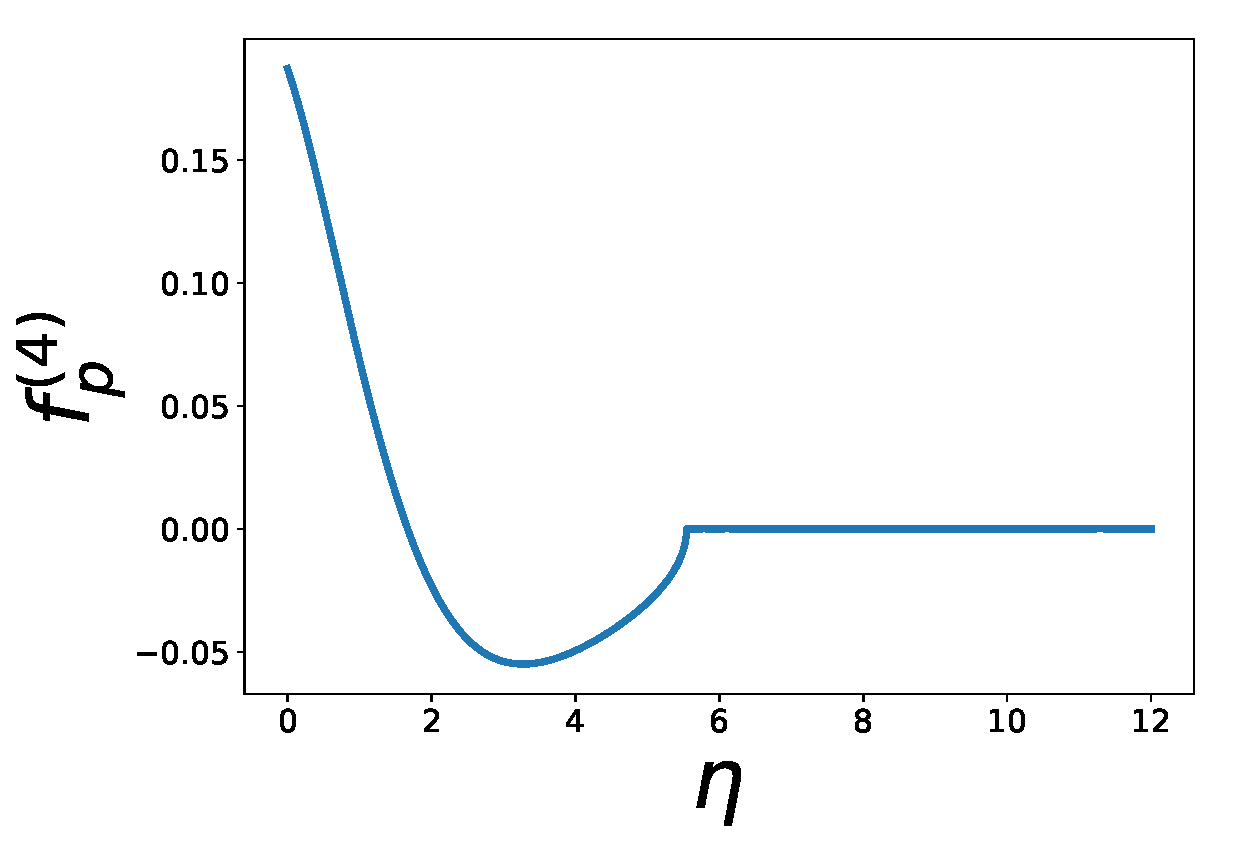
\includegraphics[width=\linewidth]{new_thickening_deriv.eps}
      \end{center}
      \footnotesize Fourth derivative of the Sakiadis separatrix solution, $\alpha=1.4$.
  \end{columns}
\end{frame}

% =========================================================================
\begin{frame}{Wall-Shear Coefficient $\kappa_p(\alpha)$}
  \begin{columns}[T,onlytextwidth]
    \column{0.45\textwidth}
      The new Sakiadis solutions glue smoothly onto the previously known range $1/2<\alpha\leq 1$:
      \begin{itemize}
        \item $\kappa_p(\alpha)$ is \emph{continuous} across $\alpha=1/2$ and $\alpha=1$.
        \item Sakiadis and Blasius curves are qualitatively similar.
      \end{itemize}
      \vspace{0.5em}
      We will see in a moment that these $\kappa_p$ values track the Carreau wall shear in the high-shear (low-$\Renx$) limit.

    \column{0.55\textwidth}
      \begin{center}
        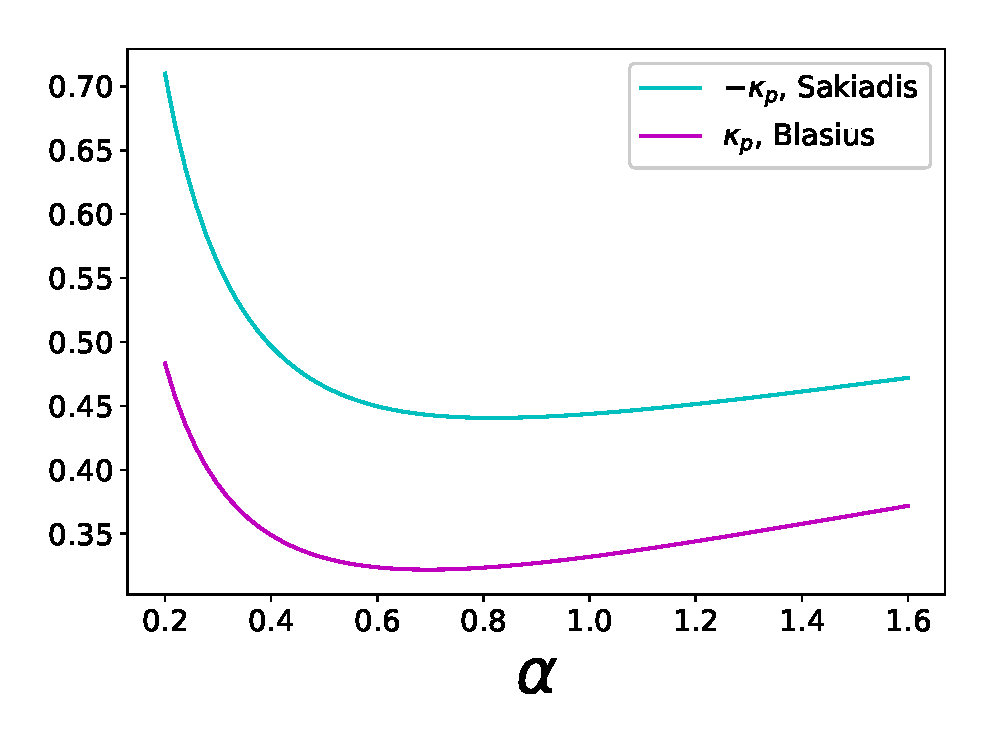
\includegraphics[width=\linewidth]{fig5.eps}
      \end{center}
  \end{columns}
\end{frame}

% =========================================================================
\begin{frame}{Wall-Shear Comparison: All Three Models}
  \begin{center}
    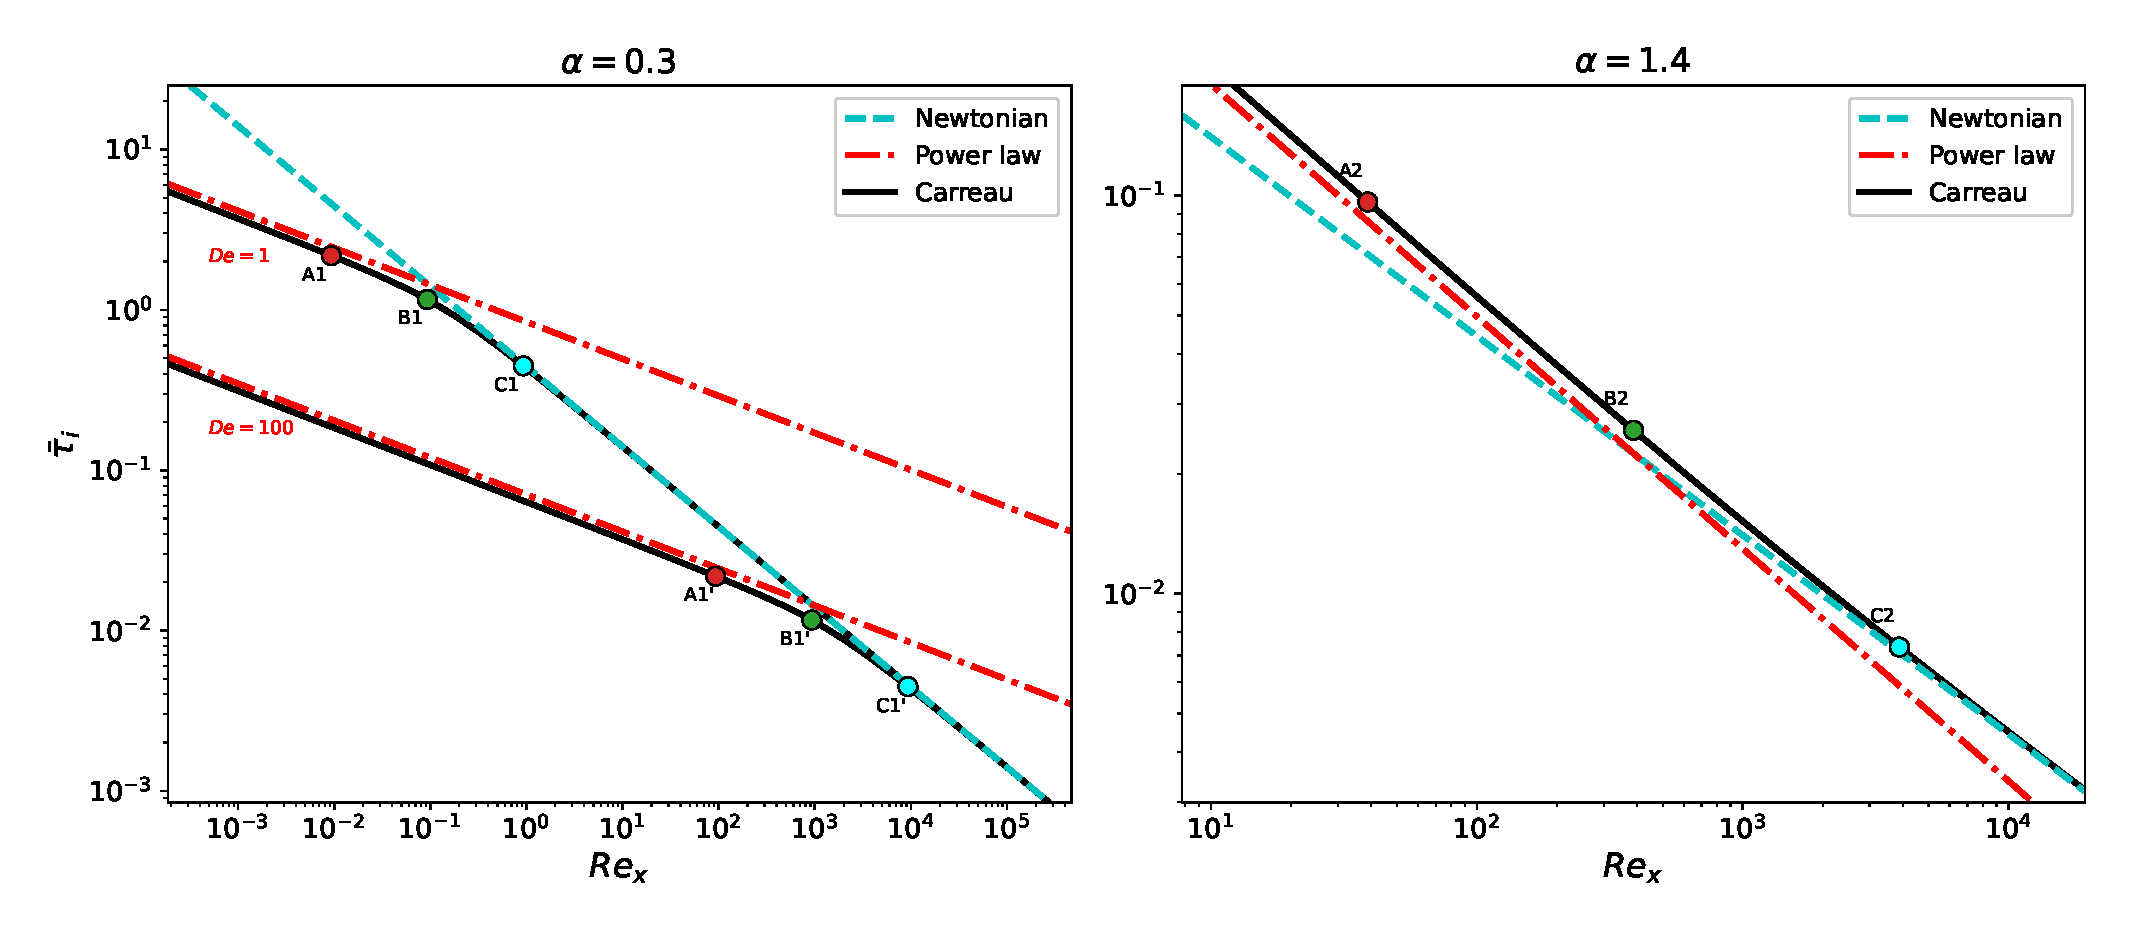
\includegraphics[width=0.78\linewidth]{new_shear.eps}
  \end{center}
  \vspace{-0.3em}
  \footnotesize
  Sakiadis wall shear vs.\ $\Renx$ at fixed $\De$, for shear-thinning ($\alpha=0.3$, multiple $\De$) and shear-thickening ($\alpha=1.4$).\\
  \textbf{Power-law line} dominates near the leading edge; \textbf{Newtonian line} dominates far downstream; Carreau bridges the two.
\end{frame}

% =========================================================================
\begin{frame}{Wall Shear: Generic Behavior}
  Across all $\alpha$, $\De$ examined (Sakiadis and Blasius):
  \begin{itemize}
    \item As $\Renx\to\infty$ (far downstream): $\delta\to0$, the Carreau ODE reduces to the Newtonian one, and
      \[
        \bar\tau_c \sim \bar\tau_n.
      \]
    \item As $\Renx\to 0$ (near leading edge):
      \[
        \bar\tau_c \sim \bigl(1-c(\alpha)\bigr)\bar\tau_p.
      \]
      The power-law line offers an excellent \emph{slope} match, but with a finite vertical offset.
  \end{itemize}
  \vspace{0.5em}
  Two key questions follow:
  \begin{enumerate}
    \item How big is the correction $c(\alpha)$, and where does it come from?
    \item Can we predict where Carreau transitions between regimes?
  \end{enumerate}
\end{frame}

% =========================================================================
\begin{frame}{The Correction $c(\alpha)$}
  \begin{columns}[T,onlytextwidth]
    \column{0.5\textwidth}
      \begin{center}
        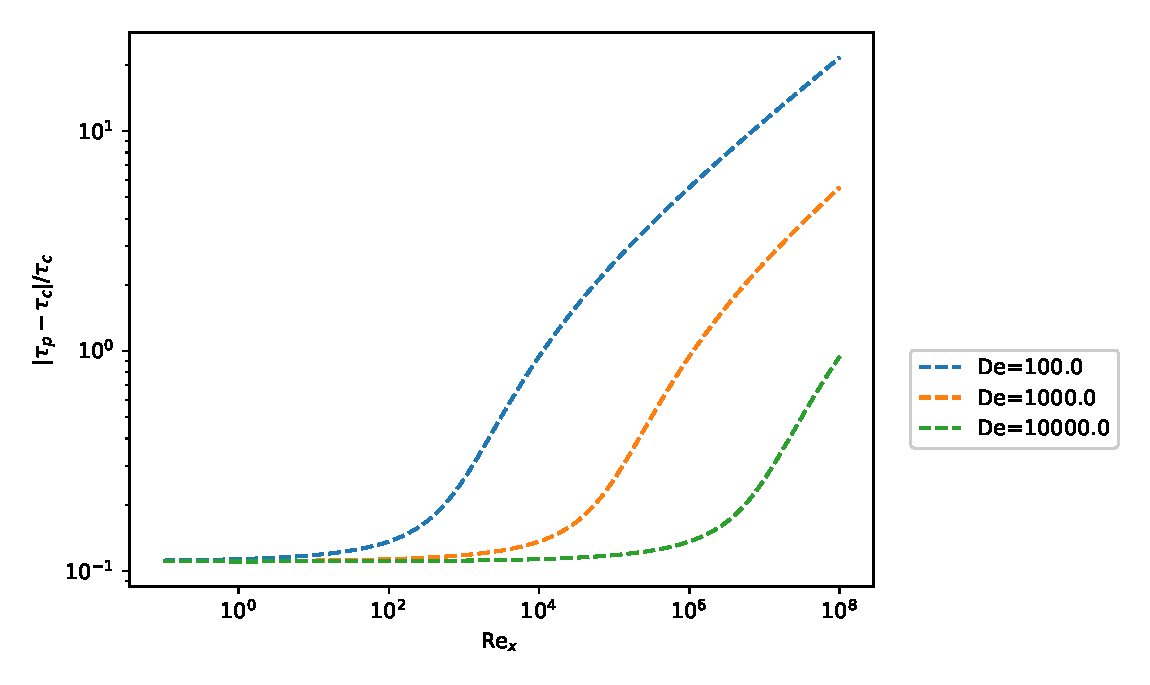
\includegraphics[width=\linewidth]{rel_err.eps}
      \end{center}
      \footnotesize Relative error $|\tau_p-\tau_c|/\tau_c$ for $\alpha=0.3$, Sakiadis flow.
    \column{0.5\textwidth}
      \begin{center}
        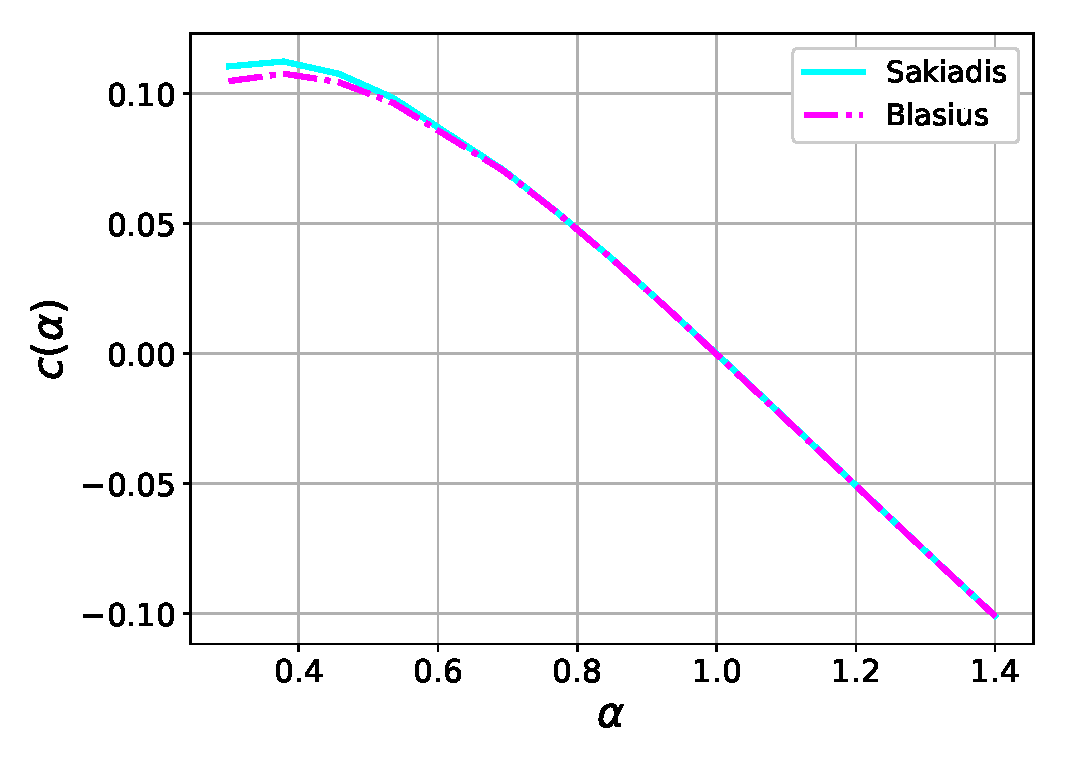
\includegraphics[width=\linewidth]{fig7.eps}
      \end{center}
      \footnotesize $c(\alpha)$ for Sakiadis and Blasius.
  \end{columns}
  \vspace{0.4em}
  \begin{itemize}
    \item Error becomes \emph{independent of $\De$} as $\Renx\to0$ --- justifying $c=c(\alpha)$.
    \item For $\alpha\in[0.3,1.4]$: $|c(\alpha)|\lesssim 11\%$.
    \item Sakiadis and Blasius corrections are \emph{essentially identical}.
  \end{itemize}
\end{frame}

% =========================================================================
\begin{frame}{Where Does $c(\alpha)$ Come From? --- Velocity Profiles}
  \begin{columns}[T,onlytextwidth]
    \column{0.55\textwidth}
      \begin{center}
        
\includegraphics[width=\linewidth]{new_profiles.eps}
      \end{center}
    \column{0.45\textwidth}
      Integrated form of the BL momentum equation:
      \[
        \bar\tau_i = \frac{\mathrm{d}}{\mathrm{d}x}\!\int_0^\infty\! u_x(U-u_x)\,\mathrm{d}y.
      \]
      The \emph{whole} velocity field affects $\bar\tau$, not just the slope at the wall.
      \vspace{0.5em}

      In the power-law regime: slopes at the wall agree, but profiles \emph{differ away from the wall} --- this is exactly the source of the residual $c(\alpha)$.
  \end{columns}
\end{frame}

% =========================================================================
\begin{frame}{A Clean Criterion: $\delta^*$}
  Setting $\bar\tau_p = \bar\tau_n$ gives the Newtonian--power-law crossover:
  \[
    \boxed{\;\delta^* = \left(\frac{\kappa_p^\alpha}{\kappa_n}\right)^{\!2(1+\alpha)/(1-\alpha)}\;}
  \]
  \begin{itemize}
    \item Both $\kappa_p(\alpha)$ and $\kappa_n$ come from \emph{self-similar} solutions only.
    \item Over $\alpha\in(0,2)$, $\delta^*$ ranges only from $\sim 14$ to $\sim 20$ --- remarkably insensitive to $\alpha$.
    \item Recipe:
      \begin{itemize}
        \item $\delta/\delta^* \gg 1$ \quad(near leading edge):\quad use power-law $\bar\tau_p$.
        \item $\delta/\delta^* \ll 1$ \quad(far downstream):\quad use Newtonian $\bar\tau_n$.
      \end{itemize}
    \item Total drag on the plate $\Rightarrow$ split the integral at $\delta=\delta^*$ --- no Carreau ODE solve needed.
  \end{itemize}
\end{frame}

% =========================================================================
\begin{frame}{Practical Takeaway}
  \begin{block}{Engineering recipe (no Carreau solver required)}
    \begin{enumerate}
      \item Look up $\kappa_p(\alpha)$ and $\kappa_n=f_p''(0;1)$ from self-similar solutions.
      \item Compute $\delta^*$ from the formula on the previous slide.
      \item Convert to a critical $x^*$ via $\delta = \lambda^2 U^3\rho/(\mu_0 x)$.
      \item Use $\bar\tau_p$ upstream of $x^*$ and $\bar\tau_n$ downstream of $x^*$.
    \end{enumerate}
  \end{block}
  \vspace{0.5em}
  \textbf{Errors with respect to the full Carreau solution:}
  \begin{itemize}
    \item $\sim 11\%$ at most in the power-law regime, attributable to $c(\alpha)$.
    \item Asymptotically zero in the Newtonian regime.
    \item Intermediate (transition) region: largest error --- the place to use the Carreau ODE if accuracy demands it.
  \end{itemize}
\end{frame}

% =========================================================================
\begin{frame}{Connections to Prior Work}
  \textbf{Denier \&\ Dabrowski (2004)}: Blasius shear-thickening solutions lose smoothness because the BL
  approximation itself breaks down where viscosity is small. They introduce a ``viscous diffusion layer''
  to recover continuity.
  \vspace{0.6em}

  \textbf{Our finding:} restoring a Newtonian plateau at low shear (i.e., the Carreau model)
  yields a completely smooth solution \emph{without} modifying the boundary-layer equation.
  \vspace{0.6em}

  \textbf{And:} the new Sakiadis power-law solutions presented here mirror the well-known
  Blasius singular structure for $\alpha>1$, completing the parallel between the two flows.
\end{frame}

% =========================================================================
\begin{frame}{Conclusions}
  \begin{enumerate}
    \item \textbf{New Sakiadis power-law solutions} for $\alpha<1/2$ (algebraic decay, $f_p\sim H(\eta+J)^p$)
          and $\alpha>1$ (finite-width boundary layer, $C^4$ but not $C^5$). Wall-shear values $\kappa_p(\alpha)$ vary continuously with $\alpha$.
    \item \textbf{Wall-shear of a Carreau fluid} is well-approximated by self-similar models in their regimes:
          \begin{itemize}
            \item Newtonian asymptote --- exact match as $\Renx\to\infty$.
            \item Power-law asymptote --- offset by a quantifiable $c(\alpha)$ ($\lesssim 11\%$ for $\alpha\in[0.3,1.4]$).
          \end{itemize}
    \item \textbf{The residual $c(\alpha)$} originates from differences in velocity profiles \emph{away from the wall},
          consistent with the integrated BL momentum balance.
    \item \textbf{A simple criterion} $\delta^*$ tells you where to switch between asymptotes ---
          giving accurate Carreau wall-shear estimates without solving the Carreau ODE family.
  \end{enumerate}
\end{frame}

% =========================================================================
\begin{frame}{Acknowledgements}
  \begin{center}
    This work was supported by the U.S.\ Department of Energy, Office of Science, Basic Energy Sciences,\\
    under Award \#\,DE-SC0025300.
    \vspace{1.5em}

    \Large Thank you --- questions?
  \end{center}
\end{frame}

\end{document}
